%
\hsection{Installing yEd on Ubuntu Linux}%
%
\begin{figure}%
\centering%
%
\subfloat[][%
We will download \yEd\ from the website \url{https://www.yworks.com/products/yed}. %
On this website, we click on the \menu{Download} button.%
\label{fig:installYedUbuntu01website}%
]{\tightbox{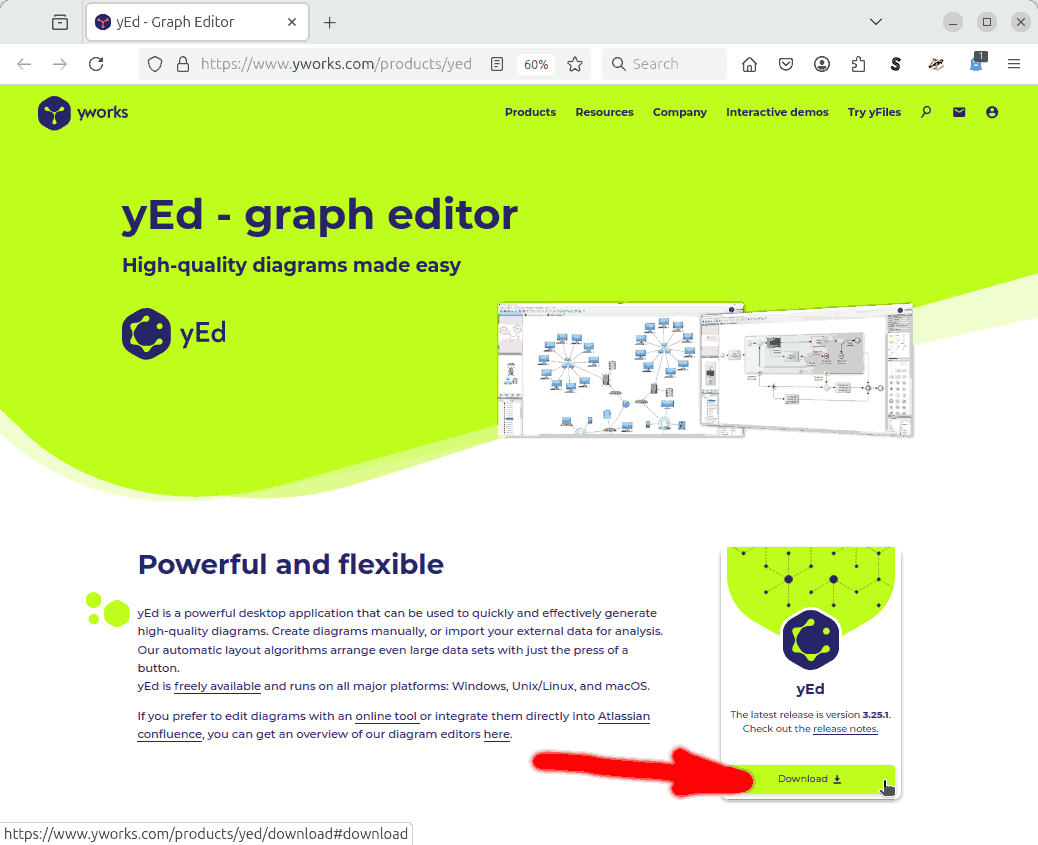
\includegraphics[width=0.48\linewidth]{\currentDir/installYedUbuntu01website}}}%
%
\floatSep%
%
\subfloat[][%
We then click on \emph{More yEd downloads}\dots%
\label{fig:installYedUbuntu02downloadsA}%
]{\tightbox{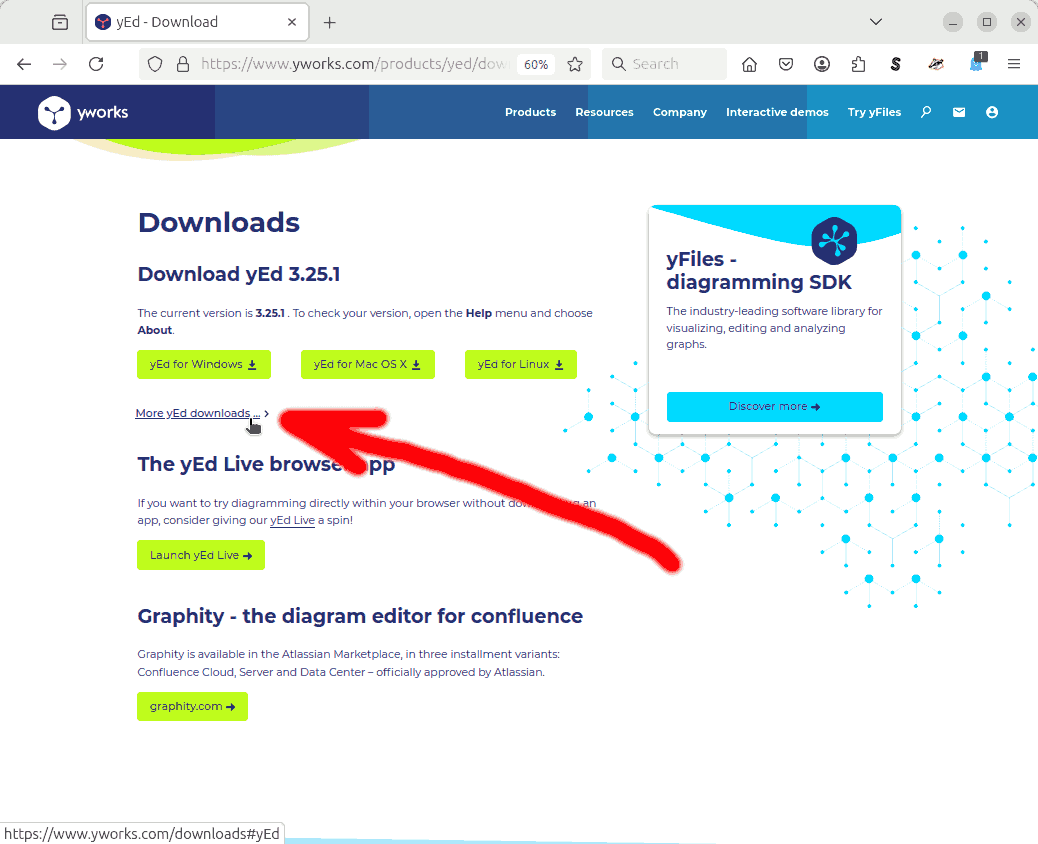
\includegraphics[width=0.48\linewidth]{\currentDir/installYedUbuntu02downloadsA}}}%
%
\floatRowSep%
%
\subfloat[][%
{\dots}and then on \emph{Show all yEd downloads}.%
\label{fig:installYedUbuntu03downloadsB}%
]{\tightbox{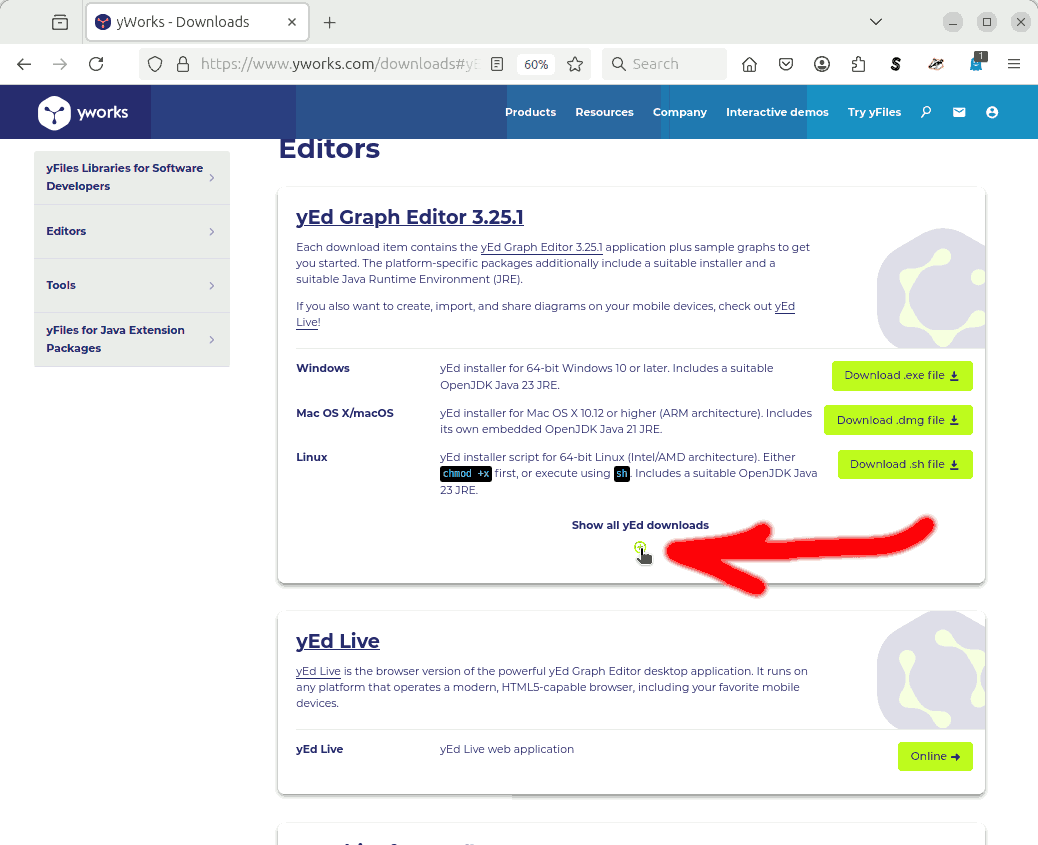
\includegraphics[width=0.48\linewidth]{\currentDir/installYedUbuntu03downloadsB}}}%
%
\floatSep%
%
\subfloat[][%
We want to download the \emph{Zipped yEd \textil{jar} file,} which is suitable for all systems that have \pgls{Java} installed. %
(If \pgls{Java} is not installed on your machine, install it via \bashil{sudo apt-get install openjdk-xx-jre}, where \textil{xx} can be replaced with the version, say \textil{8} or \textil{21}.) %
We click \menu{Download .zip file}.%
\label{fig:installYedUbuntu04downloadsC}%
]{\tightbox{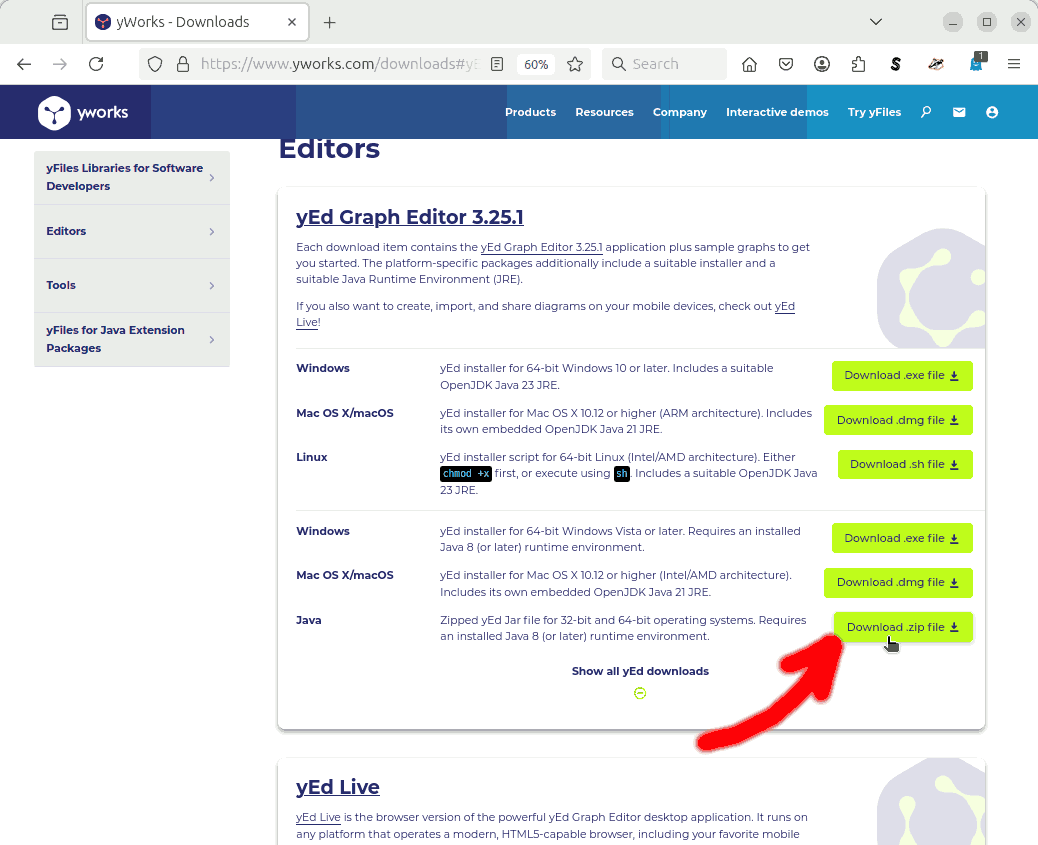
\includegraphics[width=0.48\linewidth]{\currentDir/installYedUbuntu04downloadsC}}}%
%
\caption{Installing \yEd\ under \ubuntu\ \linux.}%
\label{fig:installYedUbuntu:A}%
\end{figure}%
%
\begin{figure}%
\ContinuedFloat%
\centering%
%
\subfloat[][%
Once we clicked the download button, we get taken to the license screen. %
We carefully read the license and if we are OK with it, select \menu{I accept the license terms.}%
\label{fig:installYedUbuntu05license}%
]{\tightbox{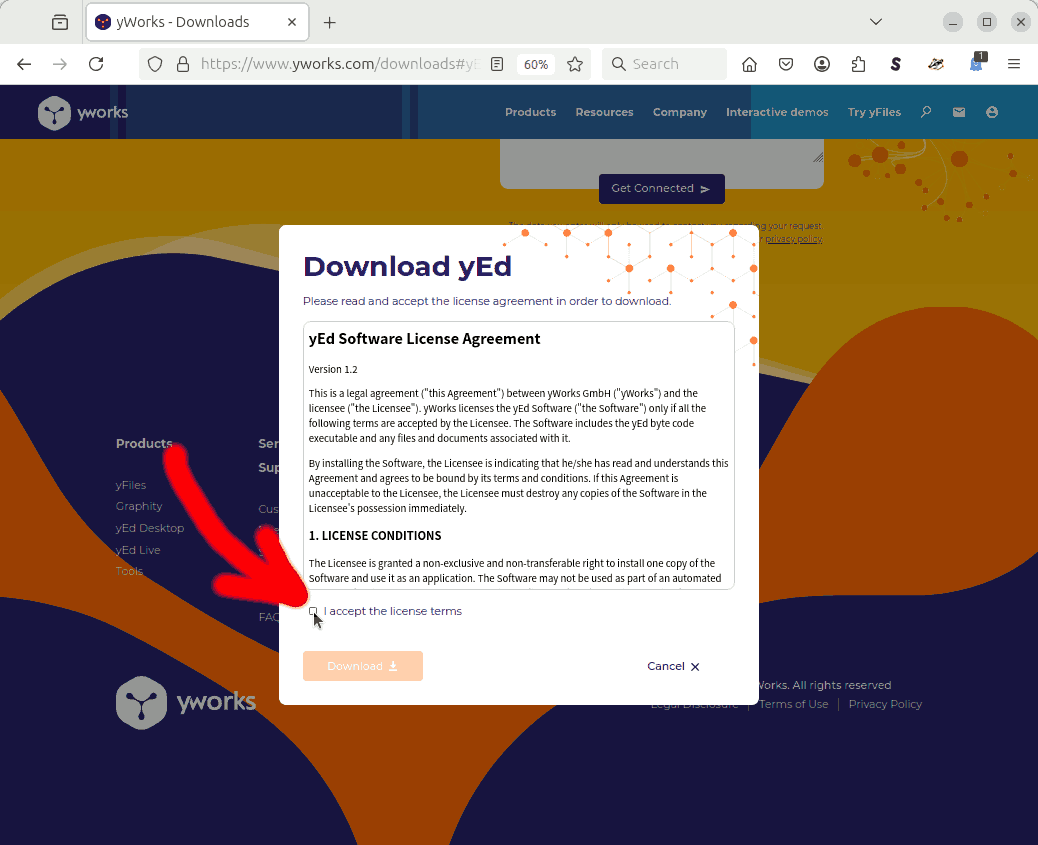
\includegraphics[width=0.48\linewidth]{\currentDir/installYedUbuntu05license}}}%
%
\floatSep%
%
\subfloat[][%
After we OKed the license, we can click on \menu{Download}.%
\label{fig:installYedUbuntu06licenseOkDownload}%
]{\tightbox{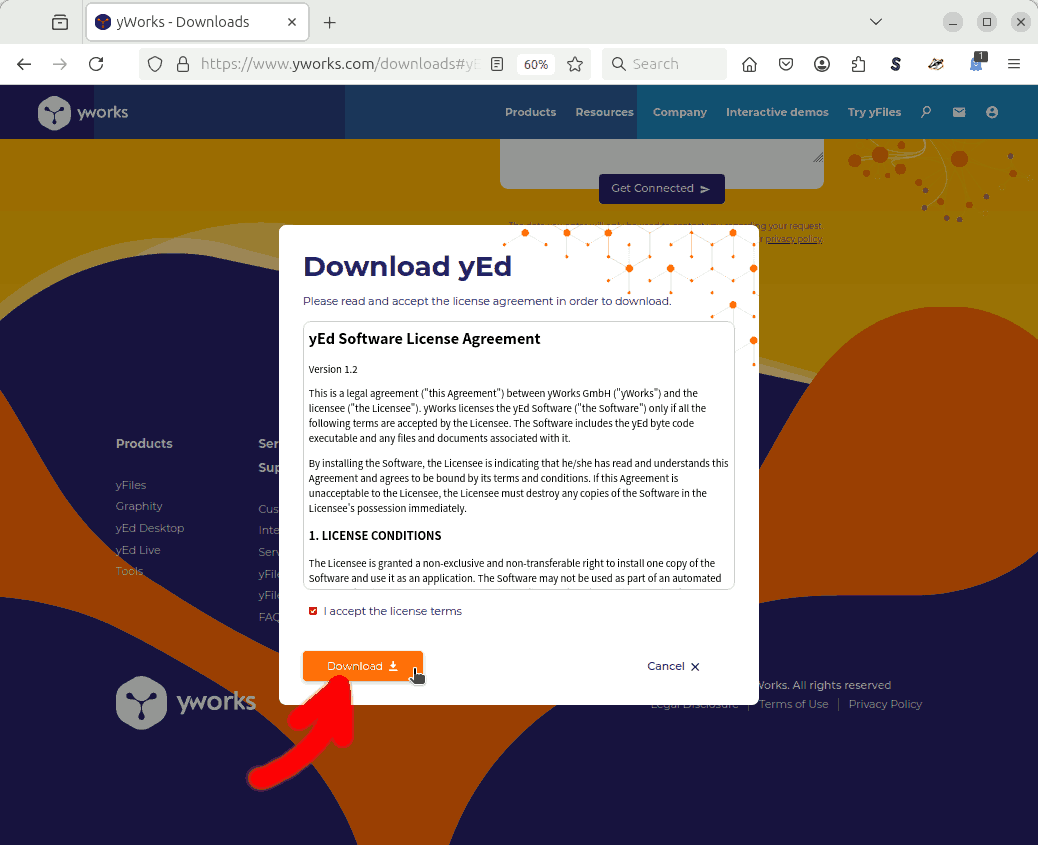
\includegraphics[width=0.48\linewidth]{\currentDir/installYedUbuntu06licenseOkDownload}}}%
%
\floatRowSep%
%
\subfloat[][%
The download starts.%
\label{fig:installYedUbuntu07downloading}%
]{\tightbox{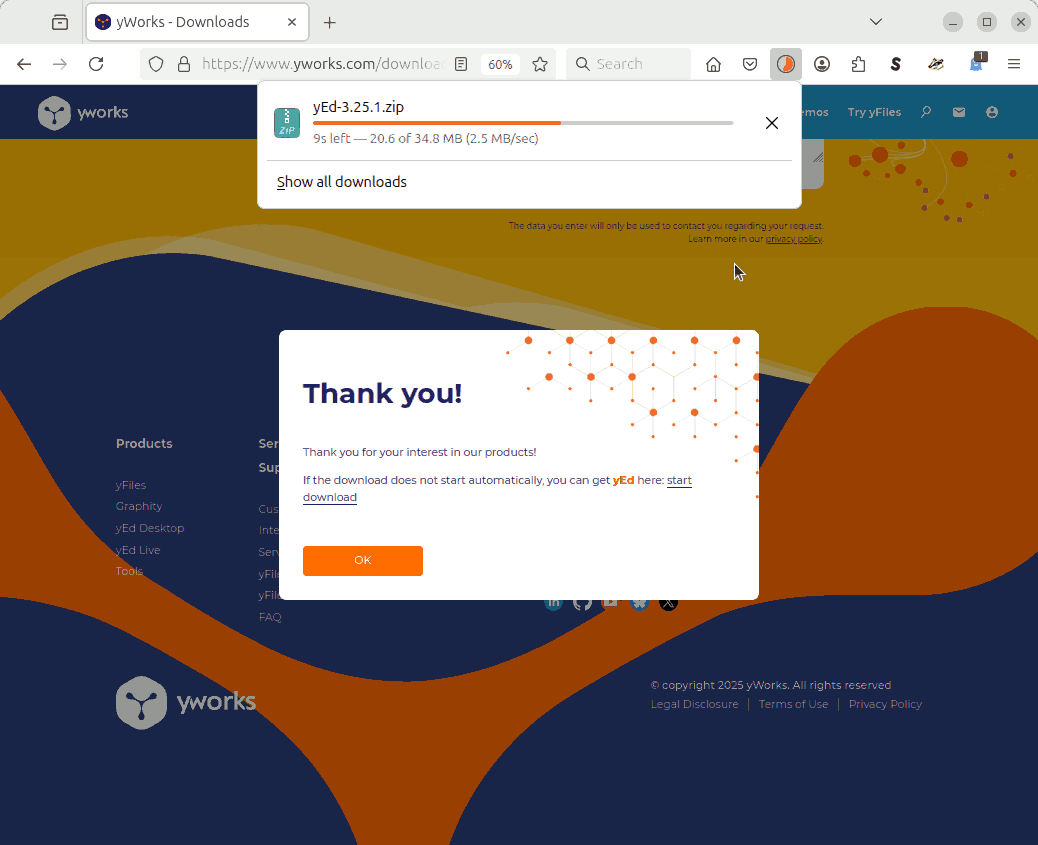
\includegraphics[width=0.48\linewidth]{\currentDir/installYedUbuntu07downloading}}}%
%
\floatSep%
%
\subfloat[][%
Eventually, the download completed. %
We can click to open the folder where the file was stored.%
\label{fig:installYedUbuntu08downloaded}%
]{\tightbox{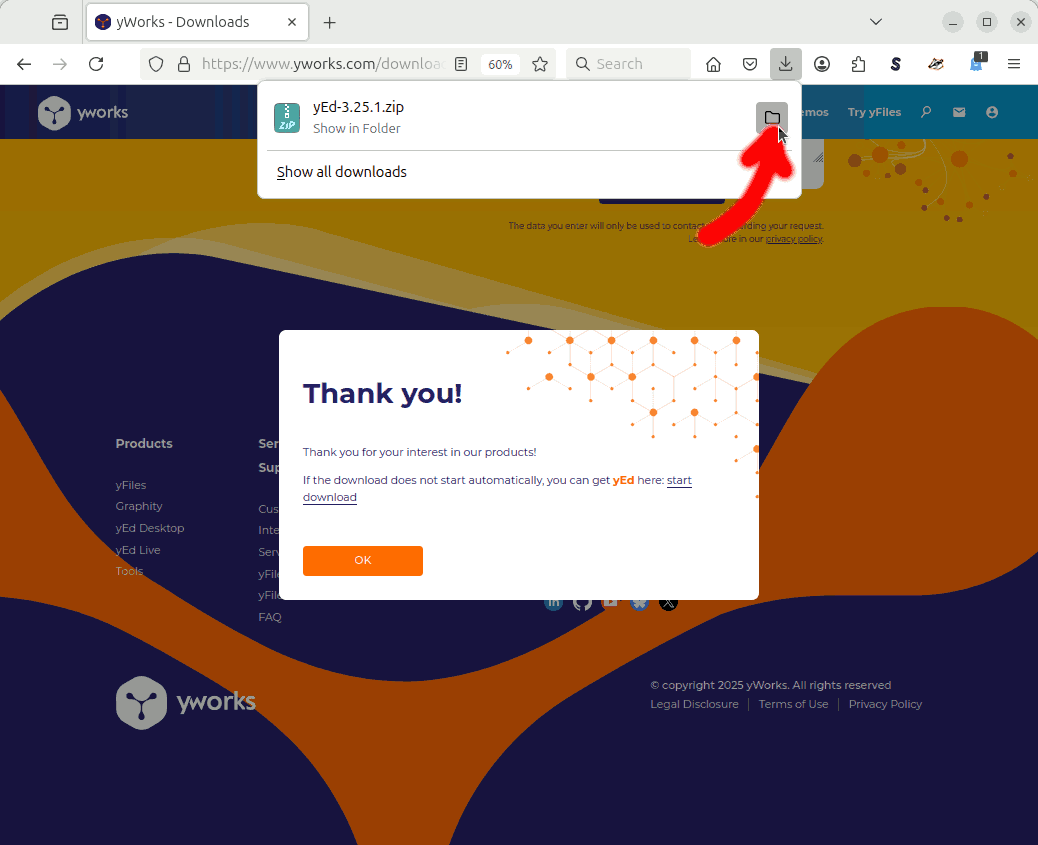
\includegraphics[width=0.48\linewidth]{\currentDir/installYedUbuntu08downloaded}}}%
%
\caption{Installing \yEd\ under \ubuntu\ \linux~(Continued).}%
\label{fig:installYedUbuntu:B}%
\end{figure}%
%
\begin{figure}%
\ContinuedFloat%
\centering%
%
\subfloat[][%
We find a \textil{zip} file in that folder. %
We unpack it to the installation location, i.e., to the place where we want to store \yEd.%
\label{fig:installYedUbuntu09inNautilus}%
]{\tightbox{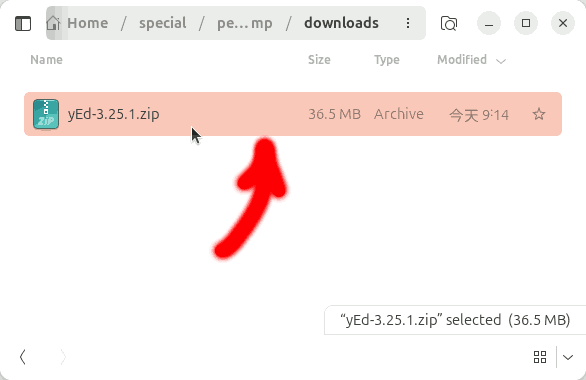
\includegraphics[width=0.48\linewidth]{\currentDir/installYedUbuntu09inNautilus}}}%
%
\floatSep%
%
\subfloat[][%
We open a console by pressing \ubuntuTerminal. %
We go to the folder which contains the unpacked data and the file \bashil{yed.jar}. %
In my case, this is \bashil{/tmp/yed}.%
\label{fig:installYedUbuntu10terminalInFodler}%
]{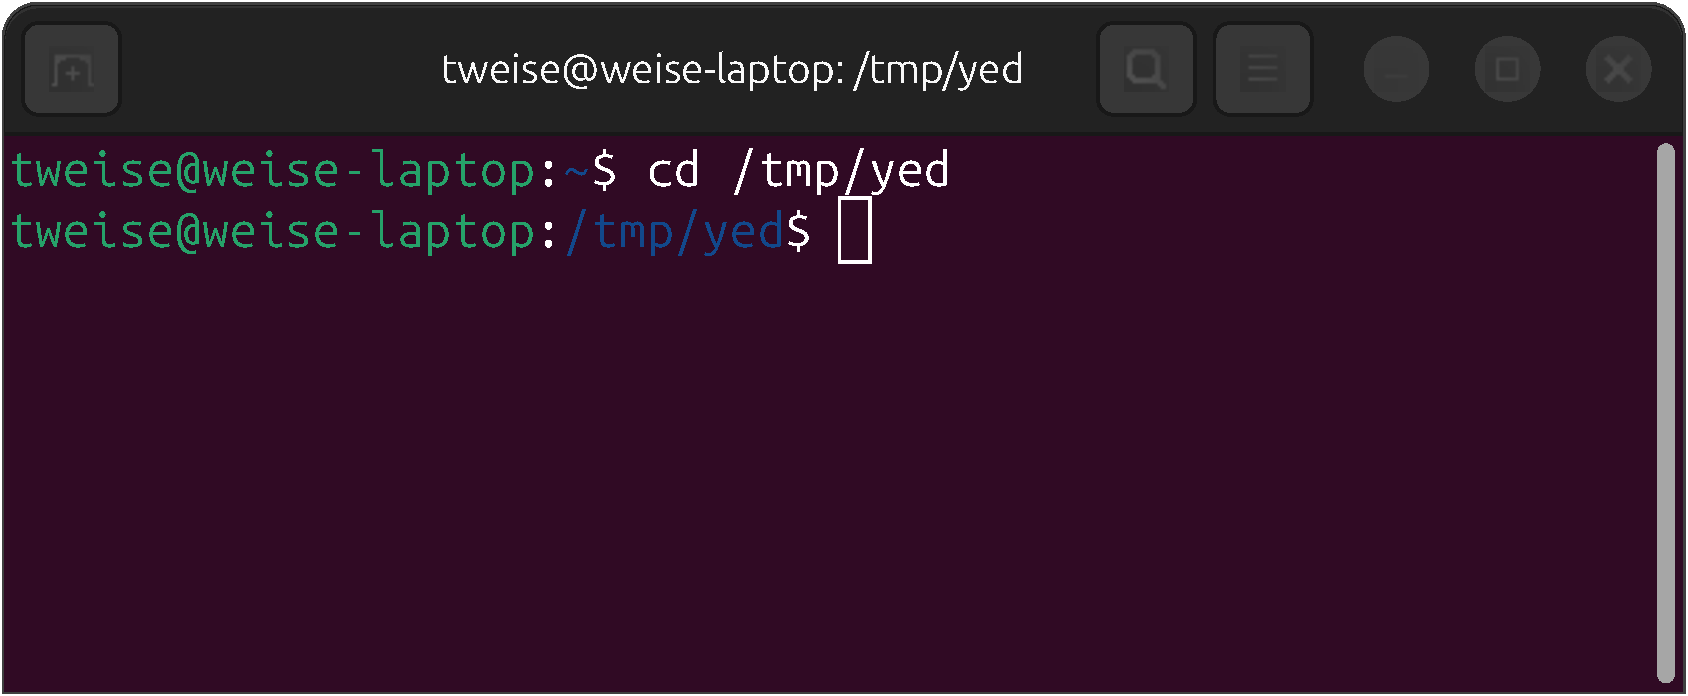
\includegraphics[width=0.48\linewidth]{\currentDir/installYedUbuntu10terminalInFolder}}%
%
\floatRowSep%
%
\subfloat[][%
We start the program by typing \bashil{java -jar yed.jar}.%
\label{fig:installYedUbuntu11javaJar}%
]{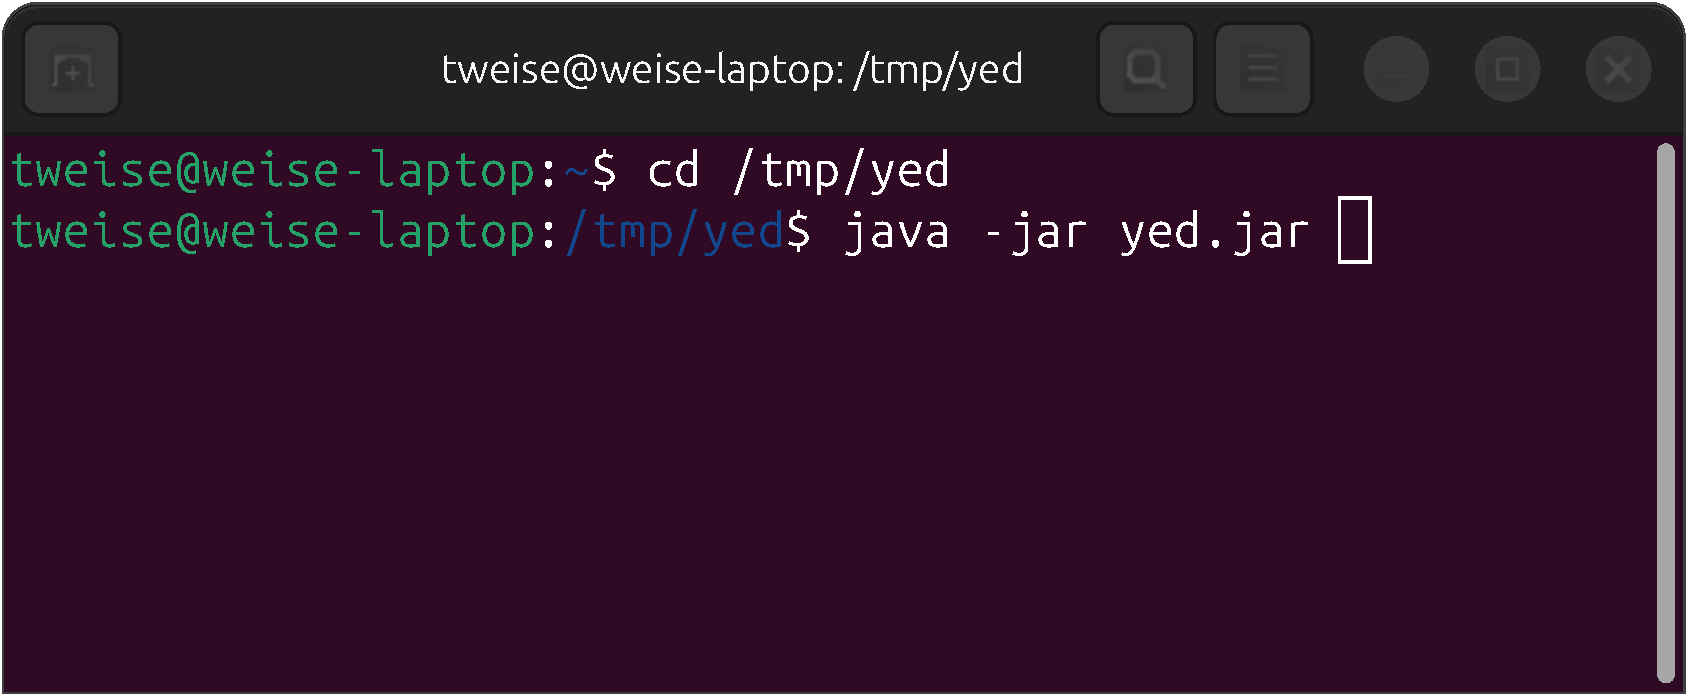
\includegraphics[width=0.48\linewidth]{\currentDir/installYedUbuntu11javaJar}}%
%
\floatSep%
%
\subfloat[][%
A splash screen appears when the program loads.%
\label{fig:installYedUbuntu12splash}%
]{\tightbox{
\includegraphics[width=0.48\linewidth]{\currentDir/installYedUbuntu12splash}}}%
%
\floatRowSep%
%
\subfloat[][%
The program has started.%
\label{fig:installYedUbuntu13yEd}%
]{\tightbox{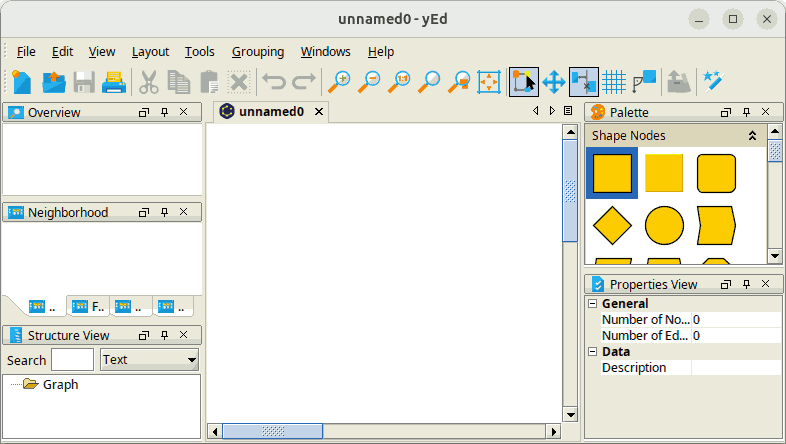
\includegraphics[width=0.75\linewidth]{\currentDir/installYedUbuntu13yEd}}}%
%
\caption{Installing \yEd\ under \ubuntu\ \linux~(Continued).}%
\label{fig:installYedUbuntu:C}%
\end{figure}%
%
In order to draw technology-independent \pglspl{ERD}, we want to install \yEd\ on our \ubuntu\ \linux\ machine.
\yEd\ is written in \pgls{Java}.
We will download the \pgls{Java} \textil{jar}~archive with the \yEd\ application together with the dependencies.
This archive can then be executed on any system that has \pgls{Java} installed and it does not require any installation.
We therefore need a \pgls{Java} installation on our machine and we then we can download the \yEd\ application.

For installing \pgls{Java}, there exist many tutorials, so we will not cover this in detail.
Installing \pgls{Java} under \ubuntu\ is fairly easy.
You would open a console \pgls{terminal} by pressing~\ubuntuTerminal.
First, you type in \bashil{java --version} to see if you already have \pgls{Java} installed.
If this command is found and produces some output, then you are done here and can directly continue with downloading \yEd.

If not, then you would type \bashil{sudo apt-get install openjdk-xx-jre}, where \textil{xx} is to be replaced with the version that you wish to install.
On my \ubuntu\ version, I can choose between \textil{8}, \textil{11}, \textil{17}, and~\textil{21}.
To see which options are available on your system, type \bashil{sudo apt-get install openjdk-} into your terminal and then press~\keys{\tab}.
This shows you a list of available installation options.
You always will want to use one that ends with~\textil{-jre}, i.e., a runtime environment~(you do not need a~\textil{-jdk}, i.e., developer kit, unless you want to write programs in \pgls{Java}, too -- which is fairly cool, so maybe you want to try this as well\dots).
I suggest to always going with the newest \textil{-jre}~version, so~\textil{21} it is in my case.
You install the newest \pgls{Java}~\bashil{jre} version on your machine.
Either way, I will assume that you have \pgls{Java} installed.

So now all we have to do is to download \yEd.
In \cref{fig:installYedUbuntu01website}, we use our browser to access the website \url{https://www.yworks.com/products/yed}.
On this website, we click on the \menu{Download} button.
In \cref{fig:installYedUbuntu02downloadsA}, we click on \emph{More yEd downloads}.
And in \cref{fig:installYedUbuntu03downloadsB}, we click on on \emph{Show all yEd downloads}.

What we want is the \textil{jar} archive with the \yEd\ application.
Therefore, we choose to download the \emph{Zipped yEd \textil{jar} file\dots} which is suitable for all systems that have \pgls{Java} installed.
We click \menu{Download .zip file} in \cref{fig:installYedUbuntu04downloadsC}.

Once we clicked the download button, we get taken to the license screen.
We carefully read the license and if we are OK with it, select \menu{I accept the license terms} in \cref{fig:installYedUbuntu05license}.
After we OKed the license, we can click on \menu{Download} in \cref{fig:installYedUbuntu06licenseOkDownload}.
The download starts in \cref{fig:installYedUbuntu07downloading}.

Eventually, the download completed.
We can click to open the folder where the file was stored in \cref{fig:installYedUbuntu08downloaded}.
We find a \textil{zip} archive in that folder.
You need to unpack this file into a proper installation location.
Notice that the \textil{zip} archive may contain a folder inside, and inside this folder, you will find the actual application.
The actual applications is the file \textil{yed.jar}, and it is bundled with several other files that you need.
So unpack the \textil{zip} archive and copy the files into the place where we want them in \cref{fig:installYedUbuntu09inNautilus}.

Since I just make these screenshots for demonstration purposes and have \yEd\ already installed elsewhere, I here choose to place the files into \bashil{/tmp/yed}.
This is \emph{not} the correct location for your installation.
You will want to choose something more permanent.

Anyway, we open a console by pressing \ubuntuTerminal.
We go to the folder which contains the unpacked data and the file \bashil{yed.jar}.
In my case, this is \bashil{/tmp/yed} in \cref{fig:installYedUbuntu10terminalInFodler}.
We start the program by typing \bashil{java -jar yed.jar} in \cref{fig:installYedUbuntu11javaJar}.

A splash screen appears when the program loads in \cref{fig:installYedUbuntu12splash}.
Finally, \cref{fig:installYedUbuntu13yEd}, the program has started.%
%
\FloatBarrier%
\endhsection%
%
